\documentclass[12pt, a4paper]{article}

\usepackage{import}
\usepackage{standalone}

\usepackage[top=4cm, right=2cm, bottom=2.7cm, left=2cm]{geometry}

\usepackage{wrapfig}
\usepackage{tabulary}
\usepackage{float}
\usepackage{pifont}
\usepackage{background}
\usepackage{tikz}


\pagestyle{empty}
\setlength{\parindent}{0pt}

\begin{document}
	\begin{minipage}{\textwidth}
		\section{Tekstmachine \hfill\small Bron: Bebras}
			
			In deze opgave gebruiken we twee soorten tekstmachines:
			
			\begin{itemize}
				\item De ''$+$'' -machine die twee stukjes tekst als invoer krijgt en als uitvoer de invoer achter elkaar plaatst.
				\item De ''$<$'' -machine die een stukje tekst als invoer krijgt en als uitvoer de tekst achterstevoren teruggeeft.
			\end{itemize}
			\begin{figure}[H]
				\raisebox{0.9\height}{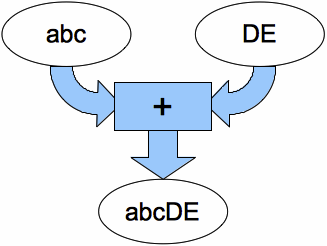
\includegraphics[width=0.4\linewidth]{image1}}
				\raisebox{0.65\height}{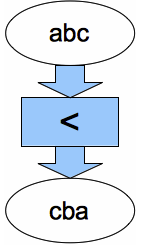
\includegraphics[width=0.2\linewidth]{image2}}		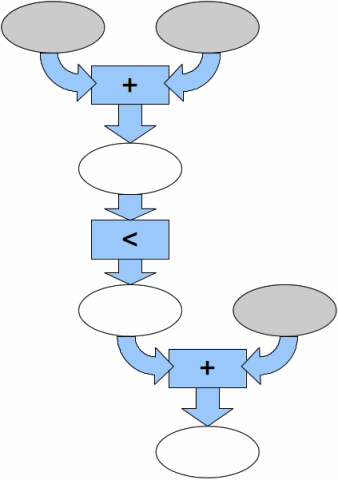
\includegraphics[width=0.4\linewidth]{image3}
			\end{figure}
	
			Door twee ''$+$'' -machines en \'e\'en ''$<$'' -machine te combineren, ontstaat een meer complexe tekstmachine (rechter afbeelding). Voor deze tekstmachine zijn drie stukjes tekst nodig als invoer (in de grijze ellipsen).
			
			Welke drie stukjes tekst (van links naar rechts) moet je als invoer geven om als uiteindelijke uitvoer ''INFORMATIE'' te krijgen?
	
			\begin{table}[H]
				\centering
				\begin{tabular}{|c|c c c|}
					\hline
					\textbf{A} & FNI  & AMRO & EIT \\
					\textbf{B} & AMR  & OFNI & EIT \\ 
					\textbf{C} & AMR  & OFNI & TIE \\ 
					\textbf{D} & INFO & RMA  & TIE \\
					\hline 
				\end{tabular}
			\end{table}
	\end{minipage} \\ \\
	
\end{document}	